\chapter{Empirical Evaluation}
This chapter contains the results from the internal evaluation of \tooln, and the results of the controlled experiment, along with the quantitative data from the experiment and post-experiment questionnaire. The results are tied to the the research questions about beneficience of \tooln~and differences between the intention-based and manual integration processes.

\section{Internal Evaluation}
The results from the internal evaluation are shown in Table \ref{tab:internalres}. We report the number of defects introduced by the developer in the merge in both tools, and the number of required editing operations for both tools. 

\begin{table}[h]
    \centering
    \caption{Internal evaluation results}
    \label{tab:internalres}
    \begin{tabular}{l|llll}
\hline\hline
\textbf{Name} & \textbf{Defects \ecl} & \textbf{Defects \inc} & \textbf{Operations \ecl} & \textbf{Operations \inc}\\
\hline
08856d9      & 0     & 0     & 4     & 1     \\
17de96a      & 1     & 2     & 13    & 5     \\
2daa859      & 2     & 5     & 14    & 5     \\
3116271      & 1     & 1     & 15    & 5     \\
373f3ec      & 4     & 3     & 35    & 7     \\
46f80e8      & 1     & 0     & 0     & 1     \\
47c1ea7      & 1     & 1     & 5     & 4     \\
\hline
esenapaj     & 5     & 2     & 271   & 185   \\ % 23 -> 2 (column err. integration)
jcrocholl    & 0     & 2     & 116   & 44    \\
STM32   & 1     & 5     & 93    & 122   \\ % 12 -> 5  (column err. integration)
\hline\hline
    \end{tabular}
\end{table}

Note that substantially fewer operations are required when using intentions, compared to the operations required when using an ordinary merge tool.

Based on the experiences from this round of evaluation, we draw three conclusions that are incorporated into the experiment design for the controlled experiment: the integration goal should be provided verbatim, rather than being described in abstract terms, cf. \cite{berger2016mps}; the tasks must be smaller so that they can be performed in a reasonable time for participants; and, subjects will require training in \tooln.


\section{Controlled Experiment}
TODO: introductory text.

\subsection{Editing Efficiency}
Figure \ref{fig:completion-times} shows the distributions of the \ctimes, with Table \ref{tab:completion-time} showing the average \ctimes, the significance tests, and effect sizes. In analogue to this, the distributions of the \eops~ is shown in Figure \ref{fig:edit-ops}, and the average \eops, significance tests, and effect sizes shown in Table \ref{tab:edit-ops}.

For \ctimes, the Mann-Whitney U-test shows a significant difference across both subject programs, with large effect sizes. We must therefore reject H1: \textit{\HA}.

For \eops, the \busybox~task shows a significant difference, while no significant difference is shown for \vim. TODO: Implications for H2: \textit{\HB}??? \todo{Thorsten: What to do about H2?}

\begin{figure}[ht]
    \centering
    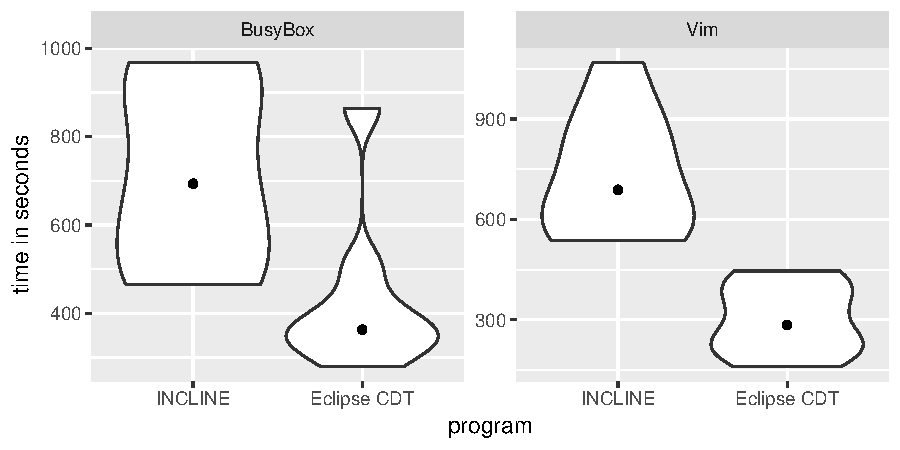
\includegraphics{figure/incl-violin-all.pdf}
    \caption{Task completion times in seconds.}
    \label{fig:completion-times}
\end{figure}

\begin{table}[ht]
    \centering
    \caption{Completion times, significance tests, and effect sizes.}
    \begin{tabular}{l | l l|l l}
    \hline
    \hline
        \textbf{Prg} & \textbf{\inc} & \textbf{\ecl} & \textbf{Significance} & \textbf{Effect size} \\\hline
        \busybox & 711 & 433 & Mann-Whitney: $W=7, p=.007$ & Cliff's delta: $d=0.78$\\
        \vim & 733 & 302 & Mann-Whitney: $W=7, p=.001$ & Cliff's delta: $d=1$\\\hline
    \hline
    \end{tabular}
    \label{tab:completion-time}
\end{table}


\begin{figure}[ht]
    \centering
    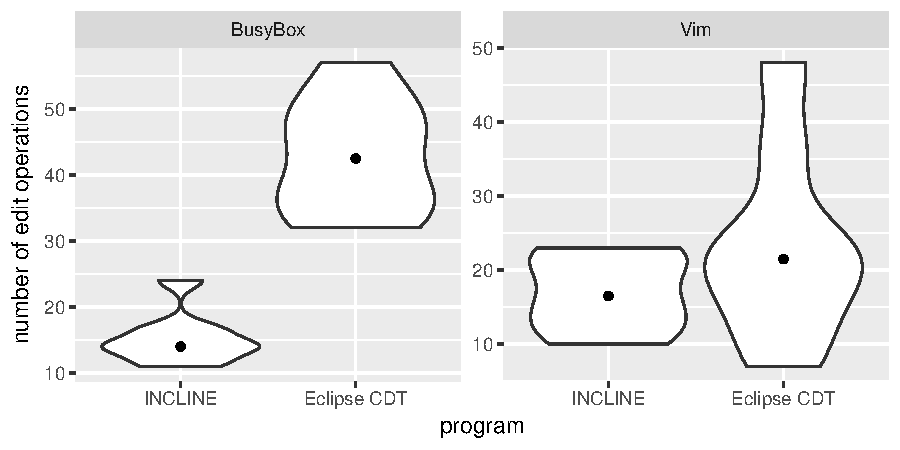
\includegraphics{figure/incl-edit-ops-violin.pdf}
    \caption{Required edit operations.}
    \label{fig:edit-ops}
\end{figure}

\begin{table}[ht]
    \centering
    \caption{Edit operations, significance tests, and effect sizes.}
    \begin{tabular}{l | l l|l l}
    \hline
    \hline
        \textbf{Prg} & \textbf{\inc} & \textbf{\ecl} & \textbf{Significance} & \textbf{Effect size} \\\hline
        \busybox & 15 & 43 & Mann-Whitney: $W=0, p= .001$ & Cliff's delta: $d=-1$\\
        \vim & 17 & 23 & Mann-Whitney: $W=23, p= .37$ & Cliff's delta: $d=-0.28$\\\hline
    \hline
    \end{tabular}
    \label{tab:edit-ops}
\end{table}

\begin{figure}[ht]
    \centering
    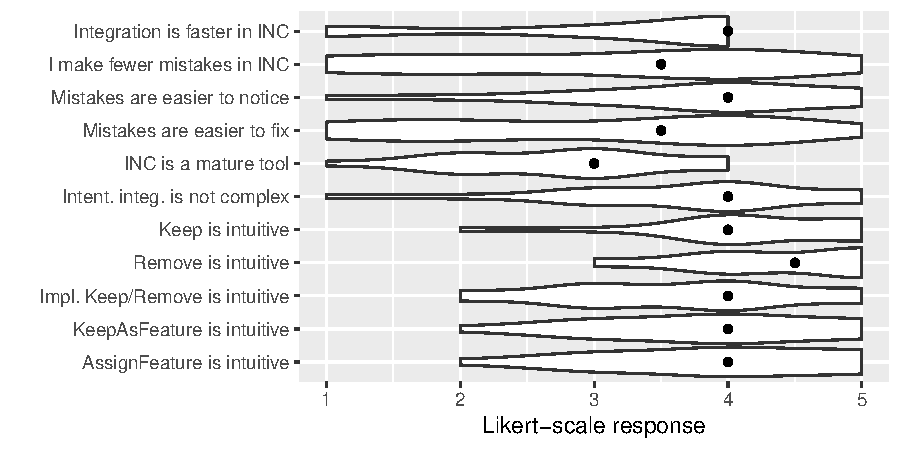
\includegraphics{figure/incl-exit-quantitative.pdf}
    1: strongly disagree, 2: disagree, 3: neutral, 4: agree, 5: strongly agree
    \caption{Post-experiment questionnaire opinions. Refer to Appendix \ref{a:questionnaires} for the full questions.}
    \label{fig:maturity}
\end{figure}

\subsection{Defects}
The number of completetely defect-free integrations is reported per program and editor in Figure \ref{fig:correct-ans}, corresponding to the zero bin in the histogram of number of defects of Figure \ref{fig:defects-hist}. For defects, we do not provide any statistical tests for significant difference between the two treatments, because of the many zero samples. Instead, we provide a graph of errors per participant in Figure \ref{fig:paricipant-errors}. \todo{Thorsten: statistical tests on number of defects, or argue from graphs that INCLINE is not worse than Eclipse?} Possibly negate hypothesis such that H3: \textit{\HC} becomes \bc Integration does NOT lead to more defects\ec.

\begin{figure}
    \centering
    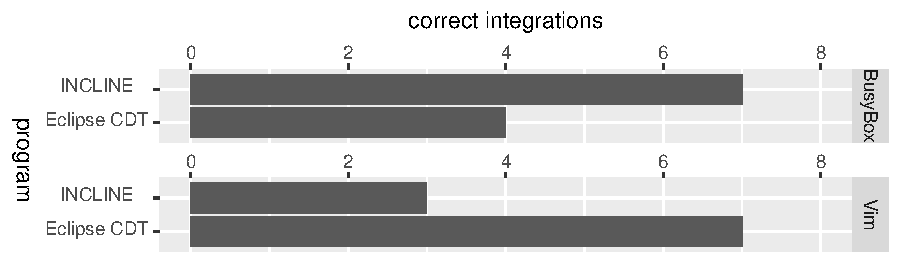
\includegraphics{figure/incl-correct-ans-r.pdf}
    \caption{Number of completely correct integrations.}
    \label{fig:correct-ans}
\end{figure}

\begin{figure}
    \centering
    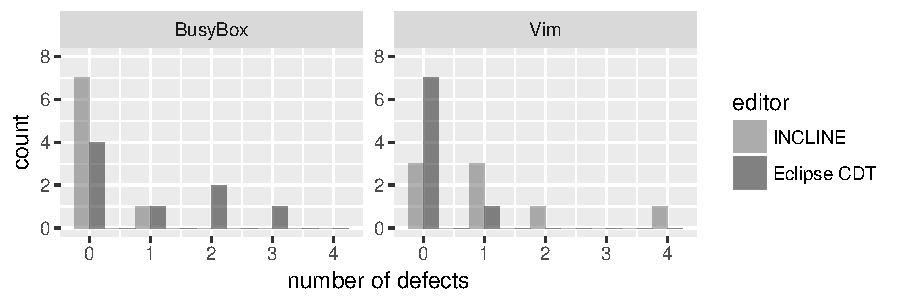
\includegraphics{figure/incl-correct-histo.pdf}
    \caption{Histogram of count of defects introduced.}
    \label{fig:defects-hist}
\end{figure}

\begin{figure}
    \centering
    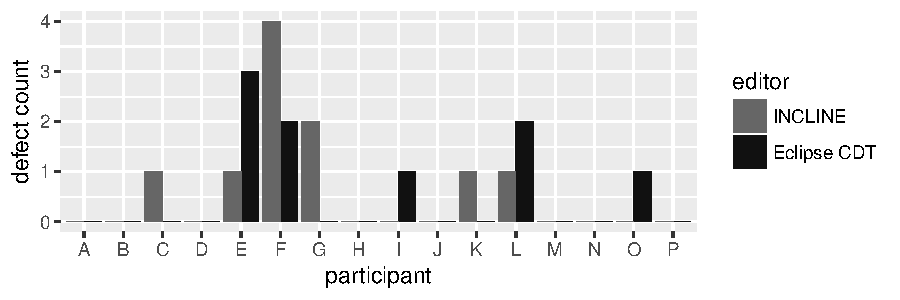
\includegraphics{figure/incl-par-errors.pdf}
    \caption{Defects per participant.}
    \label{fig:paricipant-errors}
\end{figure}


\section{\RQB}
TODO: get back to this summary once hypotheses are under control.

Recall that the overall benefit is the completion times, the edit operations, and the defects. 

There is no significant difference in the number of defects inserted between the two editors, meaning that \tooln~does not perform worse in that respect. There is however a significant difference in the required number of edit operations for one task, with a large effect size. For both tasks, there is a significant difference with respect to actual time required, with high effect sizes.

TODO: analyze the perceptions in Figure \ref{fig:maturity}.


\section{\RQC}
This section identifies differences among \tooln~and Eclipse CDT, by analyzing the open questions of the post-experiment questionnaire, screen recordings, and quantitative data from the experiment. 

\subsection{Editing}
\tooln~does not allow manual text insertion, instead relying fully on the intentions to transform the AST. Participants do not see this as a limitation, instead commending it as making the integration less-error prone (eg., \textit{\bc easier [to] avoid [...] bugs [...] and subtle differences\ec} [r3], and \textit{\bc harder to make syntatic mistakes\ec} [r11]).

A repeated criticism (or encouragement) is to create keyboard shortcuts for intentions in \tooln, to increase the editing speed.


\subsection{Intentions Semantics}
There is a noticeable tendency among participants to overselect, selecting an entire ifdef-structure, rather than the nodes inside them when applying intentions. Note that this is related to the semantics of the intentions, as opposed to editing.

Since the intentions are applied in a particular order, certain combinations of intentions will cancel out the effect completely, which leads to confusion: (eg., \textit{\bc hard to grasp how multiple conflicting intentions are prioritized\ec} [r3]). A recurring pattern is that developers apply both the \keep~and \keepasf~intentions on nodes, without any result, as the \keep~intention is an identity of the \keepasf~intention.

Overall, the perceived drawback of using \tooln~is the learning curve of the intentions semantics over the well-known paradigm of free-text editing (eg., \textit{\bc Involves a learning curve that copy and paste does not.\ec} [r14]). Compare also proficiency in free-text editing contra structured projectional editing to Berger et al. \cite{berger2016mps}.

\subsection{Integration Support}
Variant integration is given explicit concern in \tooln. The perceived benefits noted are: a) that the developer has a concrete list of all variation points that need to be integrated, and can be sure that all have been handled (eg., \textit{\bc you wont forget part of the integration\ec} [r16], and \textit{\bc It offers a nice way to work through the variabilities while making it hard to make any stupid mistakes.\ec} [r8]), b) that the views and preview help to understand the integration (eg., \textit{\bc It gives a better overview and it is easier to know where the differences are.\ec} [r7], and \textit{\bc the preview [...] and the projections [are] hugely helpful\ec} [r11]).

Participants conjecture that \tooln~is more beneficial than two-way merging in files larger than those in the tasks (eg., \textit{\bc Incline for longer periods of time and on larger projects. Manual for shorter statements.\ec} [r9], and \textit{\bc If it was a large scale project I would feel more comfortable with INCLINE.\ec} [r6]). Indeed, for future variant integration tasks, 12 respondents would prefer to use \tooln.

%\subsection{Answers to open-ended q's}
%Advantages  
%\begin{itemize}
%    \item row 4: no manual rewriting - reducing bugs and subtle differences DONE
%    \item row 7: preview reduces risk of destroying stuff
%    \item row 8: easier to locate differences
%    \item row 9: the tool does the work for you - lower chance of missing stuff
%    \item row 11: easier to keep track of what you're doing
%    \item row 12: harder to make mistakes in incline
%    \item row 13: explicit concern given to variant integration
%    \item row 15: preview?
%    \item row 17: explicitly have to deal with all variation points
%\end{itemize}

%Disadvantages
%\begin{itemize}
%    \item overall: Confusing, steep learning curve
%    \item row 10: unintuitive naming of intentions
%    \item row 13: offers no additional abstraction%
%    \item row 16: less powerful
%\end{itemize}

%Improvements
%\begin{itemize}
%    \item Useability
%    \item Unintuitive naming of intentions
%    \item Key bindings!!!!
%\end{itemize}

